\documentclass[../Cours.tex]{subfiles}

\begin{document}
\clearpage
\pagestyle{empty}

\titreDScorrection


\begin{questions}
    \EXERCICE{4}
        \question On va faire le calcul $2 \times \qty{1,20}{\EURO} + 3 \times \qty{2,20}{\EURO}$
        \question 
            \subpart{Pour les baguettes : $2 \times \qty{1,20}{\EURO} = \qty{2,40}{\EURO}$}
            \subpart{Pour les éclairs au chocolat : $3 \times \qty{2,20}{\EURO} = \qty{6,60}{\EURO}$}
            \subpart{Au total : $\qty{2,40}{\EURO} + \qty{6,60}{\EURO} = \qty{9}{\EURO}$}
        Conclusion : \textbf{Pierre va payer \qty{9}{\EURO} à la boulangerie.}

    \EXERCICE{4}
    \begin{center}
        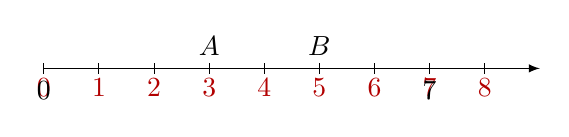
\begin{tikzpicture}[scale=0.7]
            \draw[-latex] (0,0) -- (9,0);
            \foreach \x in {0,...,8} {
                \draw (\x,-0.1) -- (\x,0.1);
                \node[red!70!black,below] at (\x,0) {$\x$};
            }
            \node at (0,-0.4) {$0$};
            \node at (7,-0.4) {$7$};
            \node at (3,0.4) {$A$};
            \node at (5,0.4) {$B$};
        \end{tikzpicture}\hspace{1cm}
        \begin{tikzpicture}[scale=0.7]
            \draw[-latex] (0,-1) -- (9,-1);
            \foreach \x in {0,...,8} {
                \draw (\x,-1.1) -- (\x,-0.9);
            }
            \foreach \x in {1,2,3,4,5,6,8} {
                \tikzmath{ integer \n; \n=\x*4; }
                \node[green!70!black,anchor=north] at (\x,-1) {$\dfrac{\n}{7}$};
            }
            \node at (0,-1.4) {$0$};
            \node at (7,-1.4) {$4$};
            \node at (2,-0.6) {$C$};
            \node at (8,-0.6) {$D$};
        \end{tikzpicture}
    \end{center}
    Réponses : $A(3)~~B(5)~~C(\dfrac{8}{7})~~D(\dfrac{32}{7})$

    \EXERCICE{4}
    \begin{center}
    \begin{tikzpicture}[scale=1]
        \draw[-latex] (0,0) -- (8,0);
        \draw[-latex] (0,0) -- (0,8);
        \foreach \x in {1,...,7} {
            \draw (\x,-0.1) -- (\x,0.1);
            \draw (-0.1,\x) -- (0.1,\x);
            \node[below] at (\x,0) {$\x$};
            \node[left] at (0,\x) {$\x$};
        };
        \node[below] at (0,0) {0};
        \coordinate (A) at (5,6);
        \coordinate (B) at (5,2);
        \coordinate (C) at (3,4);
        \coordinate (D) at (7,4);
        \coordinate (E) at (1,2);
        \coordinate (F) at (1,4);
        \coordinate (G) at (2,7);
        \coordinate (H) at (3,6);
        \coordinate (I) at (2,2);
        \draw[red] (A) -- (B) -- (C) -- (D) -- cycle;
        \draw[blue] (E) -- (F) -- (G) -- (H) -- (I) -- cycle;
        \foreach \p/\q in {A/above,B/below,C/below,D/below,E/below,F/{above left},G/above,H/above,I/below} {
            \node[\q] at (\p) {\normalsize{$\p$}};
        }
    \end{tikzpicture}
    \end{center}

    $ABCD$ a la forme d'un sablier, d'un papillon.\\
    $EFGHI$ est un \emph{pentagone} parce qu'il a 5 côtés.

    \EXERCICE{3}
        \question << Divisible par 5 >> signifie terminer par un 5 ou un 0. Il fallait donner 2 nombres parmi les suivants : 
        \begin{luacode}
for i = 10,99
do
    if i % 5 == 0
    then
        tex.print(i .. ",")
    end
end
        \end{luacode}
        \question << Divisible par 3 >> signifie que la somme des chiffres est dans la table de 3. Il fallait donner 2 nombres parmi les suivants :
        \begin{luacode}
for i = 1000,9999
do
    if i % 3 == 0
    then
        tex.print(i .. ",")
    end
end
        \end{luacode}
        \question << Divisible par 9 >> signifie que la somme des chiffres est dans la table de 9. Il fallait donner 2 nombres parmi les suivants :
        \begin{luacode}
for i = 100,999
do
    if i % 9 == 0
    then
        tex.print(i .. ",")
    end
end
        \end{luacode}

    \EXERCICE{5}
    Note : Dans la question, on demande bien de tout faire sur la même figure. Ici, pour la correction, je sépare les figures étape par étape.
    \question 
        \begin{center}
            \begin{tikzpicture}
                \coordinate (A) at (0,0);
                \coordinate (B) at (6,0);
                \draw (A) node[left] {$A$} -- (B) node[right] {$B$};
                \foreach \p in {A,B} {
                    \draw[fill=black] (\p) circle (0.05);
                }
            \end{tikzpicture}
        \end{center}
    \question 
        \begin{center}
            \begin{tikzpicture}
                \coordinate (A) at (0,0);
                \coordinate (B) at (6,0);
                \coordinate (H) at (2,0);
                \coordinate (C) at (4,1);
                \draw (A) node[left] {$A$} -- (B) node[right] {$B$};
                \foreach \p in {A,B,H,C} {
                    \draw[fill=black] (\p) circle (0.05);
                }
                \node[right] at (C) {$C$};
                \node[below] at (H) {$H$};
            \end{tikzpicture}
        \end{center}
    \question 
        \begin{center}
            \begin{tikzpicture}
                \coordinate (A) at (0,0);
                \coordinate (B) at (6,0);
                \coordinate (H) at (2,0);
                \coordinate (C) at (4,1);
                \draw (A) node[above left] {$A$} -- (B) node[right] {$B$};
                \foreach \p in {A,B,H,C} {
                    \draw[fill=black] (\p) circle (0.05);
                }
                \node[right] at (C) {$C$};
                \node[below] at (H) {$H$};
                \draw (H) -- ($(H)!1.5!(C)$);
                \draw (C) -- ($(C)!1.5!(A)$);
            \end{tikzpicture}
        \end{center}
    \question
        \begin{center}
            \begin{tikzpicture}
                \coordinate (A) at (0,0);
                \coordinate (B) at (6,0);
                \coordinate (H) at (2,0);
                \coordinate (C) at (4,1);
                \coordinate (I) at ($(H)!0.4!(C)$);
                \coordinate (J) at ($(A)!0.5!(B)$);
                \draw (A) node[above left] {$A$} -- (B) node[right] {$B$};
                \foreach \p in {A,B,H,C,I,J} {
                    \draw[fill=black] (\p) circle (0.05);
                }
                \node[right] at (C) {$C$};
                \node[below] at (H) {$H$};
                \draw (H) -- ($(H)!1.5!(C)$);
                \draw (C) -- ($(C)!1.5!(A)$);
                \node[right] at (I) {$I$};
                \node[below] at (J) {$J$};
            \end{tikzpicture}
        \end{center}
    \question 
        \begin{center}
            \begin{tikzpicture}
                \coordinate (A) at (0,0);
                \coordinate (B) at (6,0);
                \coordinate (H) at (2,0);
                \coordinate (C) at (4,1);
                \coordinate (I) at ($(H)!0.4!(C)$);
                \coordinate (J) at ($(A)!0.5!(B)$);
                \draw (A) node[above left] {$A$} -- (B) node[right] {$B$};
                \foreach \p in {A,B,H,C,I,J} {
                    \draw[fill=black] (\p) circle (0.05);
                }
                \node[right] at (C) {$C$};
                \node[below] at (H) {$H$};
                \draw (H) -- ($(H)!1.5!(C)$);
                \draw (C) -- ($(C)!1.5!(A)$);
                \node[right] at (I) {$I$};
                \node[below] at (J) {$J$};
                \draw (-3,0) -- (7,0);
            \end{tikzpicture}
        \end{center}

    \EXERCICE{(bonus) 1} On souhaite déterminer le 67ème chiffre après la virgule de $\dfrac{1234}{9999}$.\\

    En utilisant la calculatrice, ou en posant la division, on remarque que :
    $\dfrac{1234}{9999} = \num{0,1234123412341234}...$

    Les mêmes quatre chiffres 1, 2, 3 et 4 se répètent à l'infini dans cet ordre.

    On pourrait écrire tous les chiffres après la virgule jusqu'au 67ème, mais ce serait assez long. Et puis, si on demandait le \num{1000000}ème chiffre après la virgule, on ne pourrait pas résonner comme cela.

    Ce que l'on peut remarquer, c'est que le 4ème chiffre après la virgule est un 4, le 8ème aussi, le 12ème aussi, le 16ème aussi. On comprend que, si le numéro du chiffre après la virgule est un \emph{multiple} de 4, alors c'est un 4.

    En particulier, 64 est un multiple de 4 ($64 = 4 \times 16$), donc le 64ème chiffre après la virgule est un 4. Donc le 65ème est un 1, le 66ème est un 2 et le 67ème est un 3.
\end{questions}
\clearpage
\pagestyle{plain}

\end{document}